\documentclass[semifinal]{cpecmu}

%% This is a sample document demonstrating how to use the CPECMU
%% project template. If you are having trouble, see "cpecmu.pdf" for
%% documentation.

\projectNo{P008-2}
\acadyear{2022}

\titleTH{แคปสแนป : ระบบจัดการการซื้อ-ขายในร้านค้าปลีกอัตโนมัติด้วยตนเองโดยใช้ปัญญาประดิษฐ์}
\titleEN{CapSnap : Retail self-checkout system using Computational Intelligence Technique}

\author{นายพงศกร รัตนพันธ์}{Pongsakorn Rattanapan}{630610749}
\author{นางสาวศุภริฎา ศิลปสิทธิ์}{Suparida Silpasith}{690610969}

\cpeadvisor{sansanee}
\cpecommittee{kasemsit}
\committee{รศ.ดร.\,นิพนธ์ ธีรอำพน}{Assoc.\,Prof.\,Nipon Theera-Umpon, Ph.D.}

%% Some possible packages to include:
\usepackage[final]{graphicx} % for including graphics

%% Add bookmarks and hyperlinks in the document.
\PassOptionsToPackage{hyphens}{url}
\usepackage[colorlinks=true,allcolors=Blue4,citecolor=red,linktoc=all]{hyperref}
\def\UrlLeft#1\UrlRight{$#1$}

%% Needed just by this example, but maybe not by most reports
\usepackage{afterpage} % for outputting
\usepackage{pdflscape} % for landscape figures and tables. 

%% Some other useful packages. Look these up to find out how to use
%% them.
% \usepackage{natbib}    % for author-year citation styles
% \usepackage{txfonts}
% \usepackage{appendix}  % for appendices on a per-chapter basis
% \usepackage{xtab}      % for tables that go over multiple pages
% \usepackage{subfigure} % for subfigures within a figure
% \usepackage{pstricks,pdftricks} % for access to special PostScript and PDF commands
% \usepackage{nomencl}   % if you have a list of abbreviations

%% if you're having problems with overfull boxes, you may need to increase
%% the tolerance to 9999
% \tolerance=9999

\bibliographystyle{plain}
% \bibliographystyle{IEEEbib}

% \renewcommand{\topfraction}{0.85}
% \renewcommand{\textfraction}{0.1}
% \renewcommand{\floatpagefraction}{0.75}

%% Example for glossary entry
%% Need to use glossary option
%% See glossaries package for complete documentation.
\ifglossary
  \newglossaryentry{lorem ipsum}{
    name=lorem ipsum,
    description={derived from Latin dolorem ipsum, translated as ``pain itself''}
  }
\fi

%% Uncomment this command to preview only specified LaTeX file(s)
%% imported with \include command below.
%% Any other file imported via \include but not specified here will not
%% be previewed.
%% Useful if your report is large, as you might not want to build
%% the entire file when editing a certain part of your report.
% \includeonly{chapters/intro,chapters/background}

\begin{document}
\maketitle
\makesignature

\ifproject
\begin{abstractTH}
    \enskip แคปแสนป(CapSnap) เป็นระบบจัดการการซื้อ-ขายสินค้าในร้านค้าปลีก เพื่ออำนวยความสะดวก และลดความยุ่งยากในการ
    ซื้อ-ขายสินค้าทั้งทางฝั่งลูกค้า และฝั่งร้านค้า โดยลูกค้าสามารถจัดการการซื้อสินค้าได้ด้วยตนเองผ่านทางแอปพลิเคชัน
    ในโทรศัพท์มือถือ โดยแอพลิเคชันดังกล่าวจะทำการเชื่อมต่อกับร้านค้าเมื่อลูกค้าเดินเข้าร้านค้า จากนั้นลูกค้าสามารถสแกนสินค้าที่
    ต้องการแบบเรียลไทม์ ซึ่งระบบจะใช้หลักการทาง computational intelligence เพื่อบอกรายละเอียดและราคาของสินค้าแต่ละชนิดที่ถูกแสกน
    \enskip ซึ่งจะเป็นประโยชน์ต่อคนที่มีปัญหาในการมองเห็นในการเลือกซื้อสินค้า ลูกค้าสามารถระบุรายการสินค้าได้ด้วยตนเอง
    ผ่านการเพิ่ม หรือลดสินค้าในตะกร้าของแอพลิเคชัน เมื่อลูกค้าเดินออกจากร้าน ระบบจะทำการชำระเงินให้โดยอัตโนมัติ 
    ซึ่งระบบรองรับการใช้งานแอพลิเคชันกับร้านค้าปลีกหลาย ๆร้านที่มีสินค้าแตกต่างกัน นอกจากนี้ระบบยังมี 
    \enskip Website dashboard ให้บริการสําหรับฝั่งร้านค้า เพื่อช่วยให้ร้านค้าปลีกสามารถจัดการร้านได้อย่างมีประสิทธิภาพมากขึ้นโดยสามารถจัดการ 
    และดูข้อมูลคลังสินค้า รวมถึงข้อมูลการขายสินค้าได้ในเว็บไซต์เดียว
    
\end{abstractTH}

% \begin{abstract}
% The abstract would be placed here. It usually does not exceed 350 words
% long (not counting the heading), and must not take up more than one (1) page
% (even if fewer than 350 words long).

% Make sure your abstract sits inside the \texttt{abstract} environment.
% \end{abstract}

\iffalse
\begin{dedication}
This document is dedicated to all Chiang Mai University students.

Dedication page is optional.
\end{dedication}
\fi % \iffalse

\begin{acknowledgments}
Your acknowledgments go here. Make sure it sits inside the
\texttt{acknowledgment} environment.

\acksign{2020}{5}{25}
\end{acknowledgments}%
\fi % \ifproject

\contentspage

\ifproject
\figurelistpage

\tablelistpage
\fi % \ifproject

% \abbrlist % this page is optional

% \symlist % this page is optional

% \preface % this section is optional


\pagestyle{empty}\cleardoublepage
\normalspacing \setcounter{page}{1} \pagenumbering{arabic} \pagestyle{cpecmu}

\chapter{\ifenglish Introduction\else บทนำ\fi}

\section{\ifenglish Project rationale\else ที่มาของโครงงาน\fi}
\par จากระบบการขายสินค้าในร้านค้าปลีกส่วนใหญ่ของประเทศไทย ไม่ว่าจะเป็นห้างสรรพสินค้า ซุปเปอร์มาเก็ต หรือ
ร้านค้าปลีกรายย่อยต่าง ๆ พบว่าวิธีการที่ใช้ในการชำระสินค้า คือ การชำระสินค้าที่เคาน์เตอร์ชำระเงินโดยมีพนักงานบริการ
ซึ่งข้อเสียแรกของวิธีการชำระสินค้าดังกล่าว คือ การรอชำระสินค้าที่จุดชำระเงินของร้านนั้นเสียเวลา และไม่สะดวกรวดเร็ว
ยิ่งหากต้องมีการต่อแถวรอชำระเงิน ก็จะทำให้ผู้ใช้บริการเสียเวลามากขึ้น และเสียความพึงพอใจในการใช้บริการ
รวมถึงต้องมีการจัดพื้นที่สำหรับการต่อแถวอีกด้วย ด้วยเหตุนี้ จึงควรพัฒนาเทคโนโลยีที่มาช่วยการแก้ปัญหาอย่างตรงจุด
โดยให้ลูกค้าสามารถชำระสินค้าได้ด้วยตนเอง ผ่านการเลือกซื้อสินค้าได้อย่างสะดวกสบายผ่านอุปกรณ์โทรศัพท์มือถือ

นอกจากนี้สำหรับร้านค้าปลีกรายย่อยที่มีรูปแบบการขายเป็นแบบบริการตนเอง หรือแม้กระทั่งร้านค้าปลีกที่มีพนักงานชำระเงิน
แต่ไม่มีระบบช่วยจัดการยอดขาย ก็สามารถพบปัญหาในการจัดการยอดขาย และคลังสินค้าได้ เนื่องจากพนักงาน
หรือเจ้าของร้านต้องติดตามการขายสินค้าด้วยตนเองทั้งหมด โดยจะต้องคอยนับจํานวนสินค้าที่เหลืออยู่ภายในร้านเพื่อตรวจสอบว่ามีสินค้าใดถูกขายไปแล้ว 
ทำให้เกิดความยากลำบาก และผิดพลาดได้ง่าย

ผู้จัดทําจึงพัฒนาระบบ CapSnap self-service เพื่อลดปัญหาที่เกิดจากการรอชำระเงินที่แคชเชียร์
โดยพัฒนาแอพลิเคชันสำหรับผู้ใช้งานทั่วไปที่สามารถเชื่อมต่อกับร้านค้าที่เข้าร่วมเพื่อใช้บริการการซื้อสินค้าแบบ Self-service
ที่ร้านค้านั้น ๆ โดยลูกค้าสามารถเข้าใช้งานแอพลิเคชันในโทรศัพท์มือถือแล้วทำการเลือกซื้อสินค้าผ่านฟังก์ชันการสตรีมมิ่งภาพสินค้าเพื่อ
ทราบถึงรายละเอียดของสินค้า และเพิ่มสินค้าเข้าตะกร้า โดยระบบจะใช้หลักการทางความฉลาดเชิงคำนวณ (Computational Intelligence) ในการจำแนกสินค้า
ผ่านการถ่ายทอดสดรูปสินค้า ลูกค้าสามารถชำระเงินได้ด้วยตนเองพร้อมนำสินค้าที่ซื้อออกจากร้านค้าได้เลย ซึ่งระบบจะเก็บบันทึกประวัติการขายสินค้าลง
ในฐานข้อมูลเพื่อประมวลผล และแสดงบนฝั่งเว็บไซต์สำหรับร้านค้า (Website Dashboard) ซึ่งสามารถบริการจัดการคลังสินค้า และข้อมูลการขายได้ในที่เดียว
เพิ่มประสบการณ์การใช้บริการที่ดีให้ลูกค้า และเพิ่มประสิทธิภาพในการบริหารจัดการสินค้าในร้านค้าสำหรับร้านค้าที่ต้องการให้บริการแบบ
Self-service ลดการว่าจ้างพนักงาน และต้องการเครื่องมือในการบริหารร้านค้า



\section{\ifenglish Objectives\else วัตถุประสงค์ของโครงงาน\fi}
\begin{enumerate}
    \item เพื่อพัฒนาระบบ จำแนกสินค้าจากรูปภาพโดยใช้เทคนิคความฉลาดเชิงคำนวณ
    \item เพื่อสร้างระบบเว็บไซต์ และแอปพลิเคชันสำหรับโทรศัพท์มือถือเพื่อให้ผู้ใช้งานสามารถใช้งานระบบได้
\end{enumerate}

\section{\ifenglish Project scope\else ขอบเขตของโครงงาน\fi}
ข้อมูลที่ใช้ในการฝึกระบบความฉลาดเชิงคำนวณในการแยกแยะชนิดสินค้า
เป็นชุดข้อมูลชนิดอาหาร และเครื่องดื่มสำเร็จรูปที่เก็บจากร้านค้าห้อง 422 ตึก 30 ปี คณะวิศวกรรมศาสตร์ สาขาวิชาวิศวกรรมคอมพิวเตอร์ มหาวิทยาลัยเชียงใหม่
และจากร้านค้าอื่น ๆ เพิ่มเติม
% \subsection{\ifenglish Hardware scope\else ขอบเขตด้านฮาร์ดแวร์\fi}

% \subsection{\ifenglish Software scope\else ขอบเขตด้านซอฟต์แวร์\fi}

\section{\ifenglish Expected outcomes\else ประโยชน์ที่ได้รับ\fi}
\begin{enumerate}
    \item แอปพลิเคชันสำหรับโทรศัพท์มือถือที่สามารถจำแนกสินค้าผ่านการแสกนรูปสินค้า และสามารถชำระสินค้าได้
    \item เว็บไซต์ที่สามารถแสดง และจัดการข้อมูลสินค้า รวมถึงรายงานข้อมูลการขาย เพื่อให้ร้านค้าสามารถจัดการการขายได้สะดวกยิ่งขึ้น
\end{enumerate}
\section{\ifenglish Technology and tools\else เทคโนโลยีและเครื่องมือที่ใช้\fi}
\begin{enumerate}
    \item Python และ Aiortc : สำหรับพัฒนาในส่วนของ Backend การรับข้อมูลสตรีมมิ่งจากแอพลิเคชัน การฝึกสอนโมเดล และการจำแนกสินค้าโดยไม่ต้องคอยเลือกชนิดของสินค้านั้นๆ
    \item Next.js: สําหรับการพัฒนาเว็บไซต์สำหรับร้านค้า (Website Dashboard)
    \item Flutter: สำหรับพัฒนาแอปพลิเคชันสำหรับโทรศัพท์มือถือ (Mobile Application)
    \item WebSocket: เชื่อมต่อกับแอปพลิเคชันสำหรับโทรศัพท์มือถือ เพื่อถ่ายทอดสดภาพจากกล้องโทรศัพท์มือถือไปยังส่วนระบบบริการจำแนกสินค้า
    \item Supabase: สําหรับเก็บฐานข้อมูลทั้งหมดทั้งในส่วนของแอปพลิเคชันสำหรับโทรศัพท์มือถือ และเว็บไซต์สำหรับร้านค้า

\end{enumerate}
% \subsection{\ifenglish Hardware technology\else เทคโนโลยีด้านฮาร์ดแวร์\fi}

% \subsection{\ifenglish Software technology\else เทคโนโลยีด้านซอฟต์แวร์\fi}


\section{\ifenglish Project plan\else แผนการดำเนินงาน\fi}
% \begin{table}[h]
%  
%     \begin{plan}{1}{2023}{3}{2024}
%         \planitem{1}{2023}{2}{2023}{Planning}
%         \planitem{3}{2023}{3}{2023}{Document}
%         \planitem{2}{2023}{3}{2023}{Back-end development}
%         \planitem{5}{2023}{6}{2023}{App development}
%         \planitem{11}{2023}{12}{2023}{Dashboard development}
%         \planitem{1}{2024}{3}{2024}{Testing}
%     \end{plan}

%     \caption[Planning]{Planning}
%     \label{table:Planning}
%     \end{table}
\begin{table}[h]
    \begin{center}

        \vspace{0.5cm}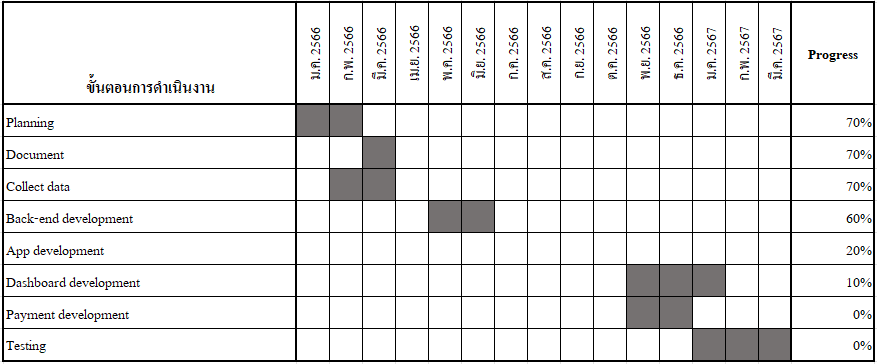
\includegraphics[scale=0.64]{pic/plane.png}
    \end{center}

    \caption[แผนการดำเนินงาน]{แผนการดำเนินงาน}
    \label{table:Planning}
\end{table}

\newpage
\section{\ifenglish Roles and responsibilities\else บทบาทและความรับผิดชอบ\fi}

\par นายพงศกร รัตนพันธ์ รหัส 630610749 มีหน้าที่ที่รับผิดชอบ ดังนี้
\begin{enumerate}
    \item การพัฒนาแอปพลิเคชันสำหรับโทรศัพท์มือถือ
    \item การรับ-ส่งข้อมูลระหว่างแอปพลิเคชันสำหรับโทรศัพท์มือถือ และระบบบริการจำแนกสินค้าผ่าน WebSocket
    \item การจัดเก็บชุดข้อมูลรูปภาพของสินค้า และการฝึกสอนโมเดลเพื่อทำระบบบริการจำแนกสินค้า
\end{enumerate}นางสาวศุภริฎา  ศิลปสิทธิ์ รหัส 630610765 มีหน้าที่ที่รับผิดชอบ ดังนี้
\begin{enumerate}
    \item การพัฒนาเว็บไซต์สำหรับร้านค้า (Website Dashboard)
    \item จัดทำระบบฐานข้อมูลทั้งหมด ทั้งในส่วนของแอปพลิเคชันสำหรับโทรศัพท์มือถือ และเว็บไซต์สำหรับร้านค้า
\end{enumerate}

\section{\ifenglish%
      Impacts of this project on society, health, safety, legal, and cultural issues
  \else%
      ผลกระทบด้านสังคม สุขภาพ ความปลอดภัย กฎหมาย และวัฒนธรรม
  \fi}

\par โครงการนี้ลดความซับซ้อน และเวลาที่ลูกค้าจะต้องรอต่อแถวเพื่อจ่ายเงินของสินค้า
% รวมถึงทำให้พนักงานของร้านค้า ไม่ต้องคอยนับจำนวนสินค้าในร้านค้า  ในร้านค้าที่เป็นระบบ Self-Service  
% อีกทั้งยังเป็นอักทางเลือกหนึ่งในการที่ร้านค้าจะมาใช้ระบบ Self-Service ที่มีการจัดการที่ดี และ ส่งเสริมวัฒนธรรมในการบริการตนเองของลูกค้า
และ เป็นจุดเริ่มต้นให้สังคมสามารถเข้าถึงเทคโนโลยีที่ก้าวหน้าไปจากเดิมในการใช้กิจวัตรประจำวันอย่างการซื้อสินค้า
โดยเปลี่ยนมาใช้การบริการตนเองผ่านแอพลิเคชันที่อำนวยความสะดวกผ่านอุปกรณ์มือถือที่ใช้งานกันอย่างแพร่หลาย
ทำให้สังคมคมก้าวสู่ความทันสมัย และความสะดวกสบายมากขึ้น ตอบโจทย์ความต้องการ และรูปแบบการใช้ชีวิตของผู้คนในยุคสมัยใหม่
ช่วยหลีกเลี่ยงปัญหาทางสุขภาพกาย ที่อาจเกิดจากการยืนรอชำระสินค้า หรือการใช้สายตาในการหาข้อมูลสินค้า
และพัฒนาสุขภาพจิตจากประสบการณ์การซื้อสินค้าที่ดีขึ้น
\par อีกทั้งยังเป็นอักทางเลือกหนึ่งในการที่ร้านค้าจะมาใช้ระบบบริการตนเองที่มีการจัดการที่ดี
เจ้าของกิจการร้านค้าปลีกสามารถจัดการบริหารร้านค้าได้สะดวก
และมีประสิทธิภาพมากขึ้น ทำให้เกิดความคุ้นเคยกับวัฒนธรรมการซื้อของแบบบริการตนเองในสังคมประเทศไทยมากขึ้น
รวมถึงเป็นต้นแบบในการพัฒนาโครงการในลักษณะเดียวกันเพื่อความก้าวหน้าทางเทคโนโลยีในประเทศต่อไป
\chapter{\ifenglish Background Knowledge and Theory\else ทฤษฎีที่เกี่ยวข้อง\fi}

% การทำโครงงาน เริ่มต้นด้วยการศึกษาค้นคว้า ทฤษฎีที่เกี่ยวข้อง หรือ งานวิจัย/โครงงาน ที่เคยมีผู้นำเสนอไว้แล้ว ซึ่งเนื้อหาในบทนี้ก็จะเกี่ยวกับการอธิบายถึงสิ่งที่เกี่ยวข้องกับโครงงาน เพื่อให้ผู้อ่านเข้าใจเนื้อหาในบทถัดๆ ไปได้ง่ายขึ้น
โครงงานนี้ได้นำองค์ความรู้ในด้านของ Computational Intelligence และ การ streaming แบบ Peer-to-peer   
ของรูปภาพจาก application ไปยัง backend ผ่าน WebRTC (Web Real Time Communications) เพื่อให้ backend 
ที่เป็น Computational Intelligence ทำการ classification products โดยโครงสร้างของระบบจะเป็นดังรูป \ref{fig:Overall project structure}
\begin{figure}[h]
  \begin{center}
  % 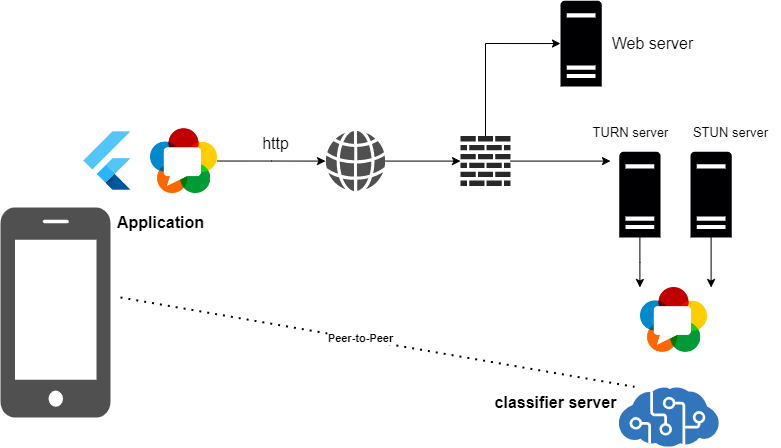
\includegraphics{pic/webrtc.png}
  \vspace{0.5cm}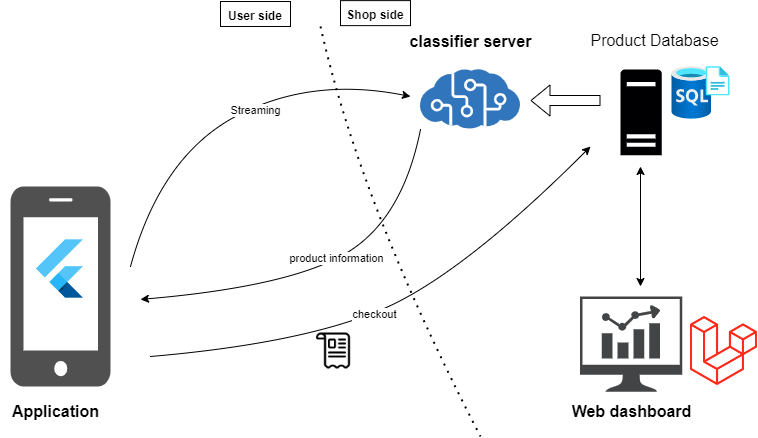
\includegraphics[scale=0.5]{pic/overall.png}
  \end{center}
  
  \caption[Overall project structure]{Overall project structure}
  \label{fig:Overall project structure}
  \end{figure}
  
  \newpage
 
\section{WebRTC for Streaming image}
WebRTC (Web Real-Time Communication) เป็น open-source  ที่ให้บริการ  web browsers
 และ mobile applications ด้วยการสื่อสารแบบเรียลไทม์ (RTC) ผ่าน (API)  
 ทำให้การ Communication ด้วยเสียงและวิดีโอได้ผ่าน  Peer-to-peer   โดยตรงตามรูป \ref{fig:webrtc structure}
 
 
\begin{figure}[h]
\begin{center}
% 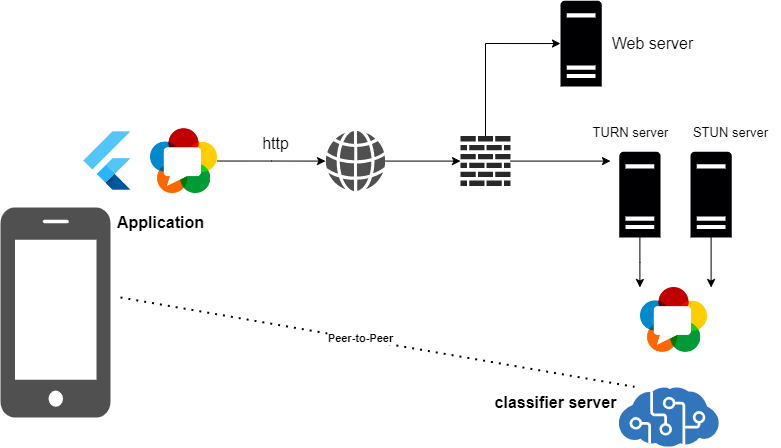
\includegraphics{pic/webrtc.png}
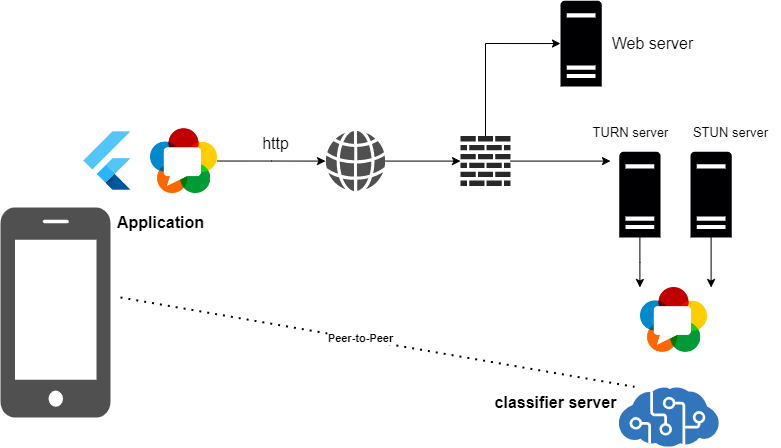
\includegraphics[scale=0.5]{pic/webrtc.png}
\end{center}

\caption[webrtc structure]{webrtc structure}
\label{fig:webrtc structure}
\end{figure}



\section{Product database}
Section 2 text.

\section{Computational Intelligence}

 
\subsection{Transfer Learning}

Subsection 1 text

\section{classification products}

\section{web dashboard}
% Section 3 text. The dielectric constant\index{dielectric constant}
% at the air-metal interface determines
% the resonance shift\index{resonance shift} as absorption or capture occurs
% is shown in Equation~\eqref{eq:dielectric}:

% \begin{equation}\label{eq:dielectric}
% k_1=\frac{\omega}{c({1/\varepsilon_m + 1/\varepsilon_i})^{1/2}}=k_2=\frac{\omega
% \sin(\theta)\varepsilon_\mathit{air}^{1/2}}{c}
% \end{equation}

% \noindent
% where $\omega$ is the frequency of the plasmon, $c$ is the speed of
% light, $\varepsilon_m$ is the dielectric constant of the metal,
% $\varepsilon_i$ is the dielectric constant of neighboring insulator,
% and $\varepsilon_\mathit{air}$ is the dielectric constant of air.

% \section{About using figures in your report}

% define a command that produces some filler text, the lorem ipsum.
% \newcommand{\loremipsum}{
%   \textit{Lorem ipsum dolor sit amet, consectetur adipisicing elit, sed do
%   eiusmod tempor incididunt ut labore et dolore magna aliqua. Ut enim ad
%   minim veniam, quis nostrud exercitation ullamco laboris nisi ut
%   aliquip ex ea commodo consequat. Duis aute irure dolor in
%   reprehenderit in voluptate velit esse cillum dolore eu fugiat nulla
%   pariatur. Excepteur sint occaecat cupidatat non proident, sunt in
%   culpa qui officia deserunt mollit anim id est laborum.}\par}

% \begin{figure}
  % \centering

  % \fbox{
    %  \parbox{.6\textwidth}{\loremipsum}
  % }

  % To include an image in the figure, say myimage.pdf, you could use
  % the following code. Look up the documentation for the package
  % graphicx for more information.
  % \includegraphics[width=\textwidth]{myimage}

  % \caption[Sample figure]{This figure is a sample containing \gls{lorem ipsum},
  % showing you how you can include figures and glossary in your report.
  % You can specify a shorter caption that will appear in the List of Figures.}
  % \label{fig:sample-figure}
% \end{figure}

% Using \verb.\label. and \verb.\ref. commands allows us to refer to
% figures easily. If we can refer to Figures
% \ref{fig:walrus} and \ref{fig:sample-figure} and \ref{fig:webrtc}  by name in the {\LaTeX}
% source code, then we will not need to update the code that refers to it
% even if the placement or ordering of the figures changes.

% \loremipsum\loremipsum

% This code demonstrates how to get a landscape table or figure. It
% uses the package lscape to turn everything but the page number into
% landscape orientation. Everything should be included within an
% \afterpage{ .... } to avoid causing a page break too early.
% \afterpage{
%   \begin{landscape}
%   \begin{table}
%     \caption{Sample landscape table}
%     \label{tab:sample-table}

%     \centering

%     \begin{tabular}{c||c|c}
%         Year & A & B \\
%         \hline\hline
%         1989 & 12 & 23 \\
%         1990 & 4 & 9 \\
%         1991 & 3 & 6 \\
%     \end{tabular}
%   \end{table}
%   \end{landscape}
% }

% \loremipsum\loremipsum\loremipsum

% \section{Overfull hbox}

% When the \verb.semifinal. option is passed to the \verb.cpecmu. document class,
% any line that is longer than the line width, i.e., an overfull hbox, will be
% highlighted with a black solid rule:
% \begin{center}
% \begin{minipage}{2em}
% juxtaposition
% \end{minipage}
% \end{center}

% \section{\ifenglish%
% \ifcpe CPE \else ISNE \fi knowledge used, applied, or integrated in this project
% \else%
% ความรู้ตามหลักสูตรซึ่งถูกนำมาใช้หรือบูรณาการในโครงงาน
% \fi
% }

% อธิบายถึงความรู้ และแนวทางการนำความรู้ต่างๆ ที่ได้เรียนตามหลักสูตร ซึ่งถูกนำมาใช้ในโครงงาน

% \section{\ifenglish%
% Extracurricular knowledge used, applied, or integrated in this project
% \else%
% ความรู้นอกหลักสูตรซึ่งถูกนำมาใช้หรือบูรณาการในโครงงาน
% \fi
% }

% อธิบายถึงความรู้ต่างๆ ที่เรียนรู้ด้วยตนเอง และแนวทางการนำความรู้เหล่านั้นมาใช้ในโครงงาน

\chapter{\ifproject%
\ifenglish Project Structure and Methodology\else โครงสร้างและขั้นตอนการทำงาน\fi
\else%
\ifenglish Project Structure\else โครงสร้างของโครงงาน\fi
\fi
}

ในบทนี้จะกล่าวถึงหลักการ และการออกแบบระบบ

\makeatletter

% \renewcommand\section{\@startsection {section}{1}{\z@}%
%                                    {13.5ex \@plus -1ex \@minus -.2ex}%
%                                    {2.3ex \@plus.2ex}%
%                                    {\normalfont\large\bfseries}}

\makeatother
%\vspace{2ex}
% \titleformat{\section}{\normalfont\bfseries}{\thesection}{1em}{}
% \titlespacing*{\section}{0pt}{10ex}{0pt}

\section{ชุดข้อมูลฝึกสอน}


\section{model}



% \begin{figure}[h]
% \begin{center}
% % 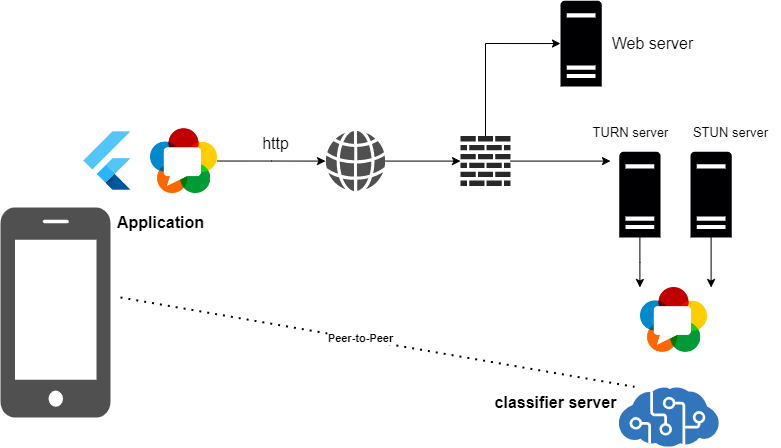
\includegraphics{pic/webrtc.png}
% 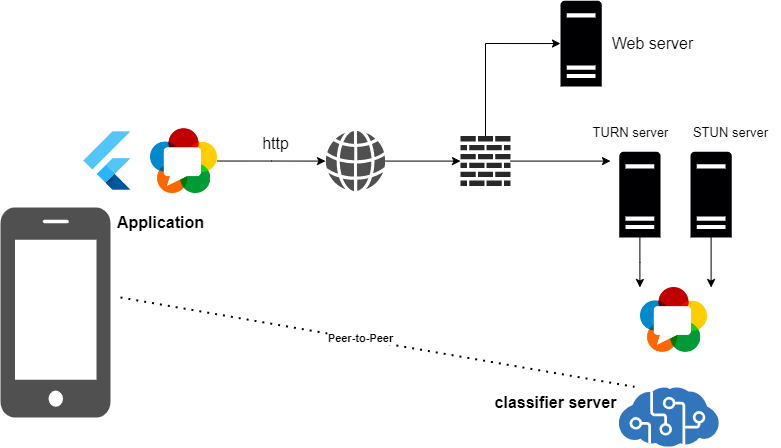
\includegraphics[scale=0.5]{pic/webrtc.png}
% \end{center}

% \caption[webrtc structure]{webrtc structure}
% \label{fig:webrtc structure}
% \end{figure}
\newpage
\section{การพัฒนาเว็บไซด์}

\section{แผนภาพกระแสข้อมูล (Data Flow Diagram)}
\begin{figure}[h]
  \begin{center}
  % 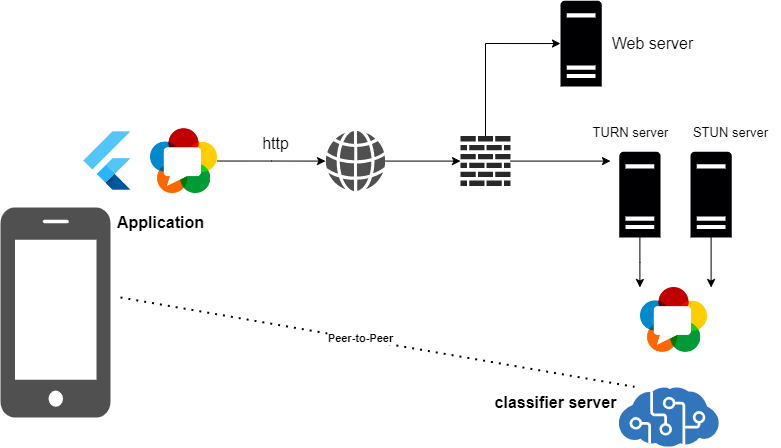
\includegraphics{pic/webrtc.png}
  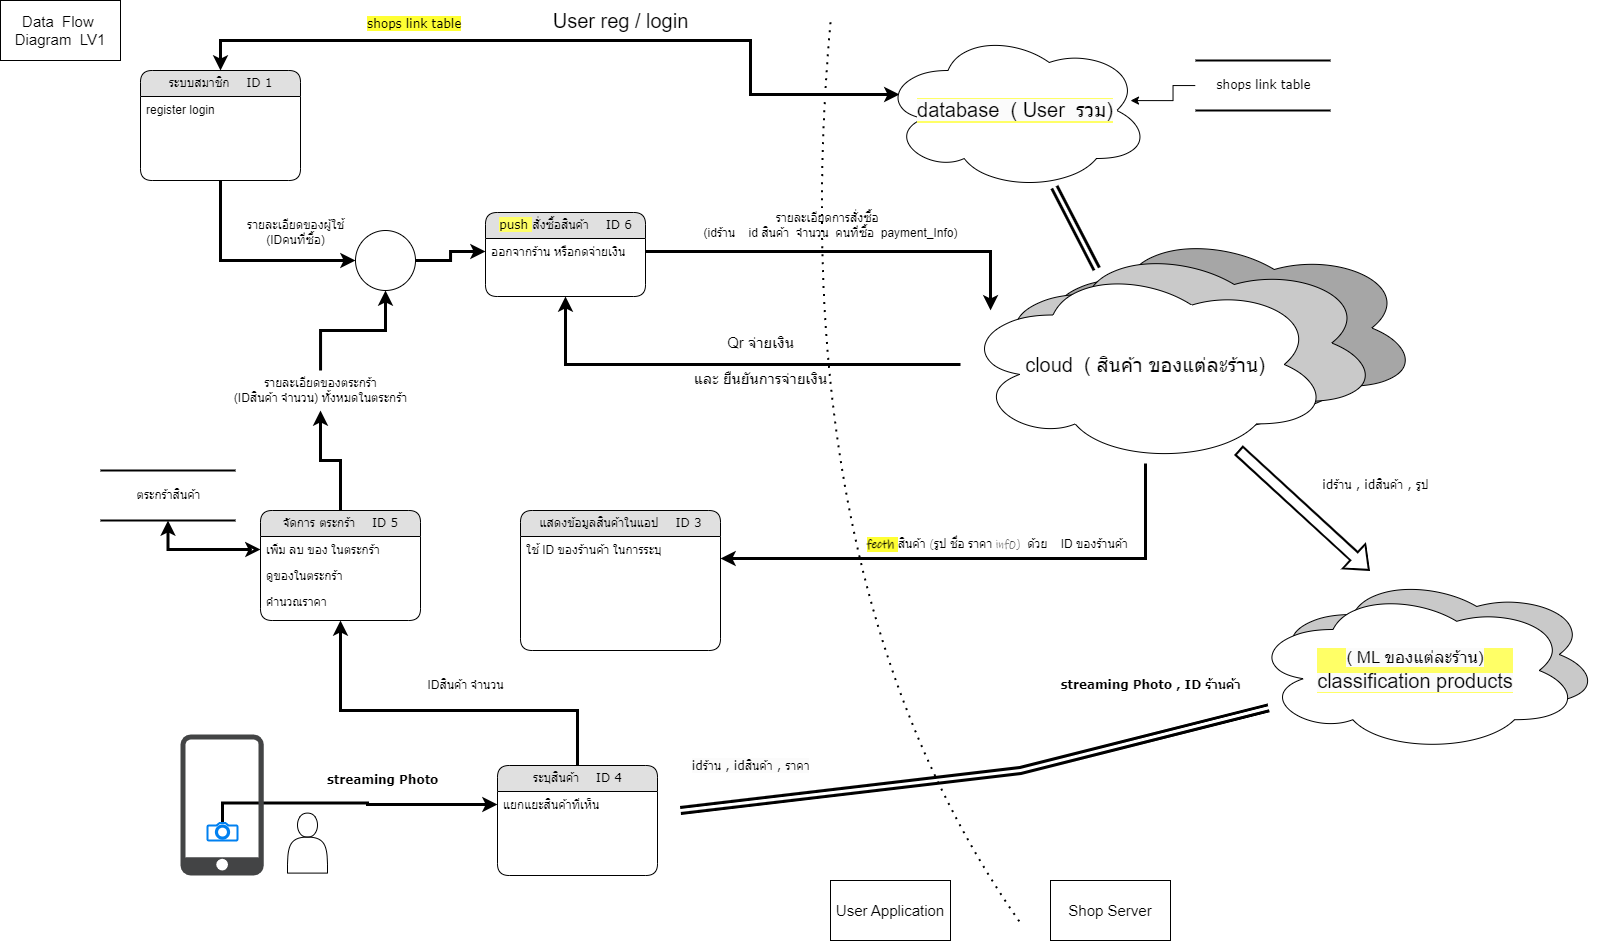
\includegraphics[scale=0.25]{pic/dataflow-lv0.png}
  \end{center}
  
  \caption[Data Flow Diagram]{Data Flow Diagram}
  \label{fig:Data Flow Diagram}
  \end{figure}
  

% \subsection{The Black Kitten}
  % One thing was certain, that the WHITE kitten had had nothing to
% do with it:---it was the black kitten's fault entirely



% ~\cite{aiw}. 




%  For the
% white kitten had been having its face washed by the old cat for
% the last quarter of an hour (and bearing it pretty well,
% considering); so you see that it COULDN'T have had any hand in
% the mischief.

%   The way Dinah washed her children's faces was this:  first she
% held the poor thing down by its ear with one paw, and then with
% the other paw she rubbed its face all over, the wrong way,
% beginning at the nose:  and just now, as I said, she was hard at
% work on the white kitten, which was lying quite still and trying
% to purr---no doubt feeling that it was all meant for its good.

%   But the black kitten had been finished with earlier in the
% afternoon, and so, while Alice was sitting curled up in a corner
% of the great arm-chair, half talking to herself and half asleep,
% the kitten had been having a grand game of romps with the ball of
% worsted Alice had been trying to wind up, and had been rolling it
% up and down till it had all come undone again; and there it was,
% spread over the hearth-rug, all knots and tangles, with the
% kitten running after its own tail in the middle.

% \subsection{The Reproach}

  
\chapter{\ifproject%
\ifenglish Experimentation and Results\else การทดลองและผลลัพธ์\fi
\else%
\ifenglish System Evaluation\else การประเมินระบบ\fi
\fi}

\section{Application UX/UI}
 
\begin{figure}[h]
    \begin{center}
    % 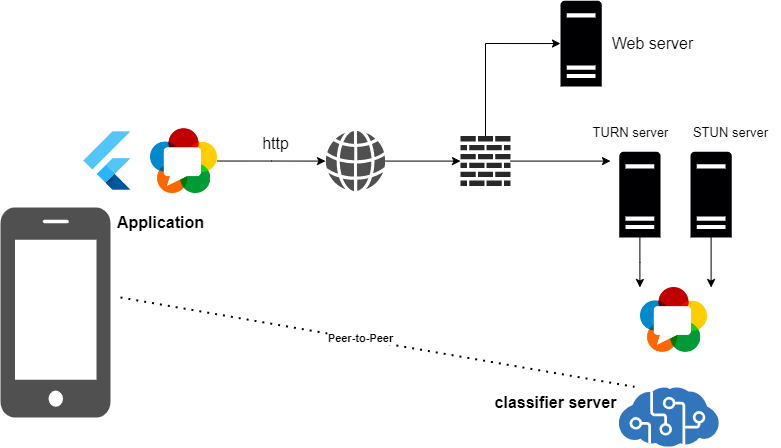
\includegraphics{pic/webrtc.png}
    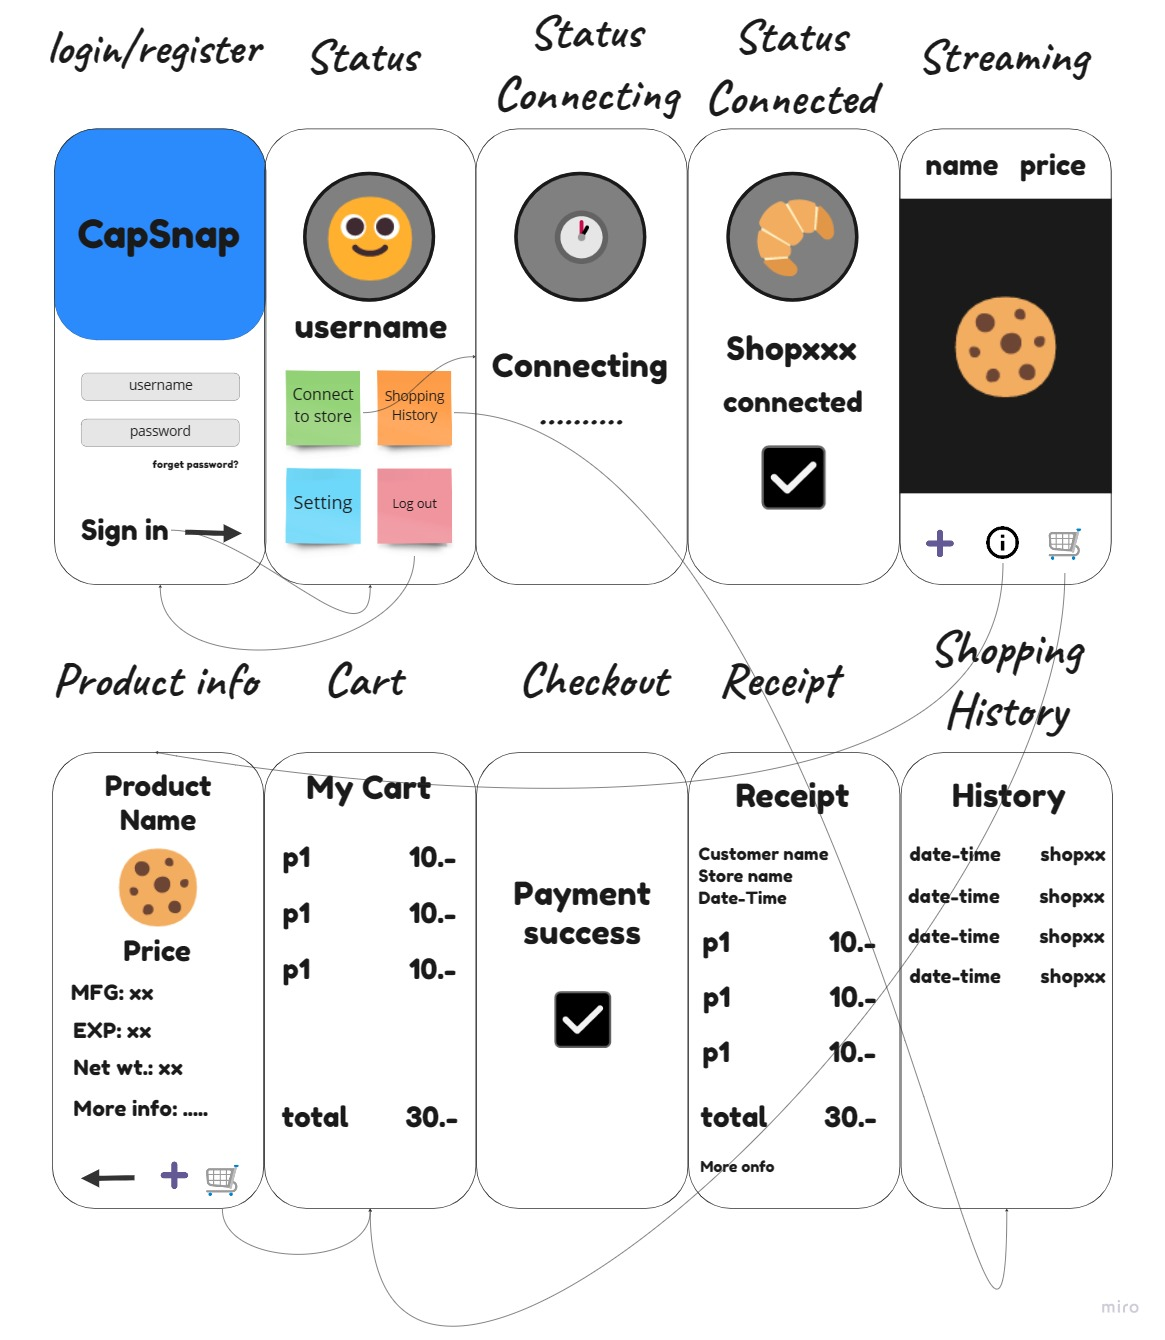
\includegraphics[scale=0.25]{pic/ui/mobileui.jpg}
    \end{center}
    
    \caption[Application wire frame]{Application wire frame}
    \label{fig:Application wire frame}
    \end{figure} 

    \section{Web Dashboard UX/UI}
    % \begin{center}
{
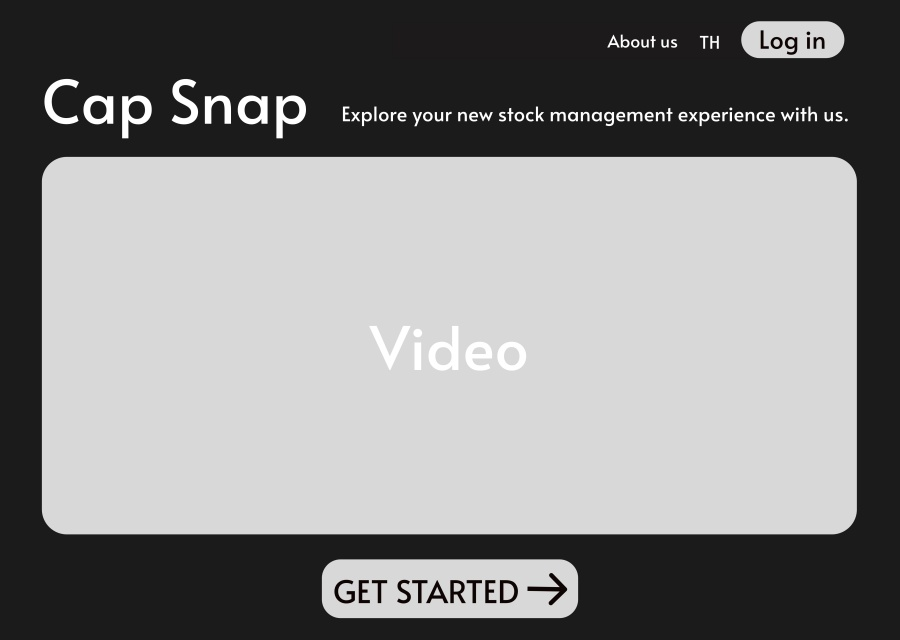
\includegraphics[scale=0.9]{pic/ui/1.jpg}
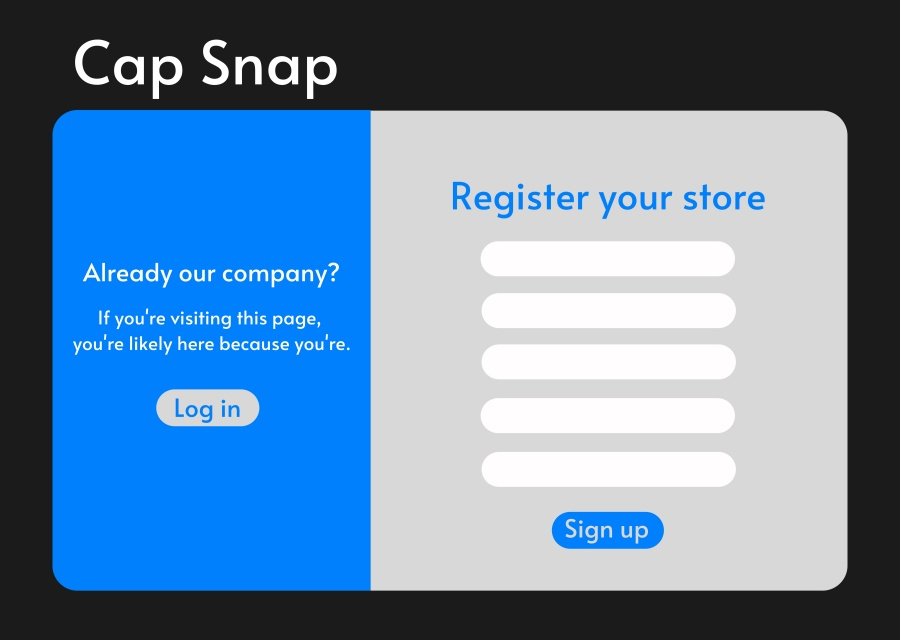
\includegraphics[scale=0.9]{pic/ui/2.jpg}
}\\
{
 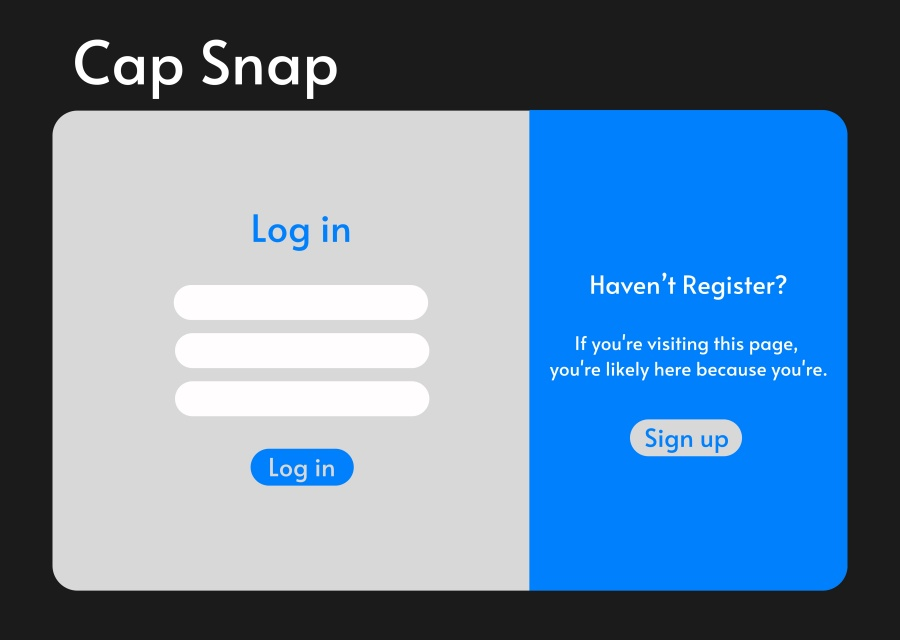
\includegraphics[scale=0.9]{pic/ui/3.jpg}
 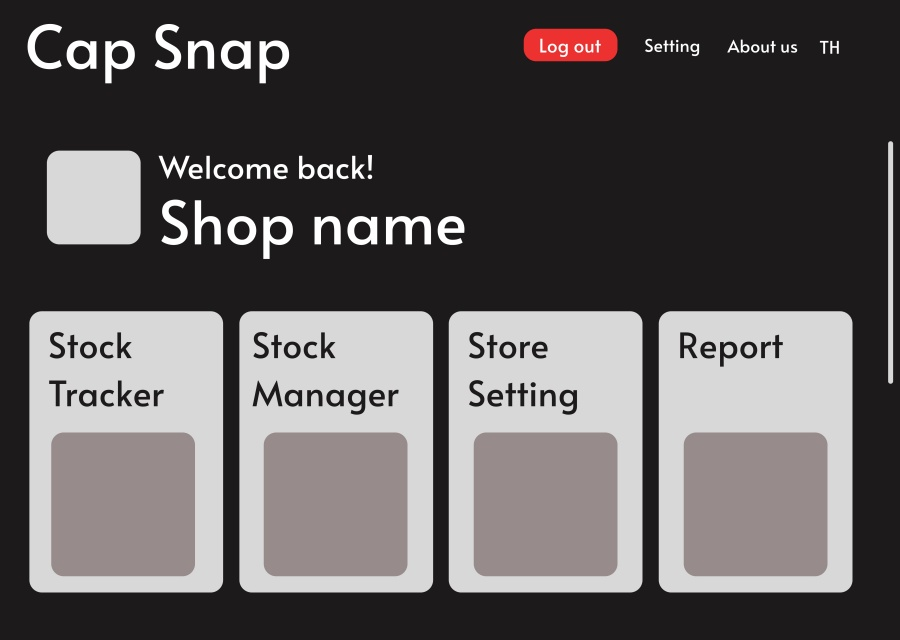
\includegraphics[scale=0.9]{pic/ui/4.jpg}
}\\
{
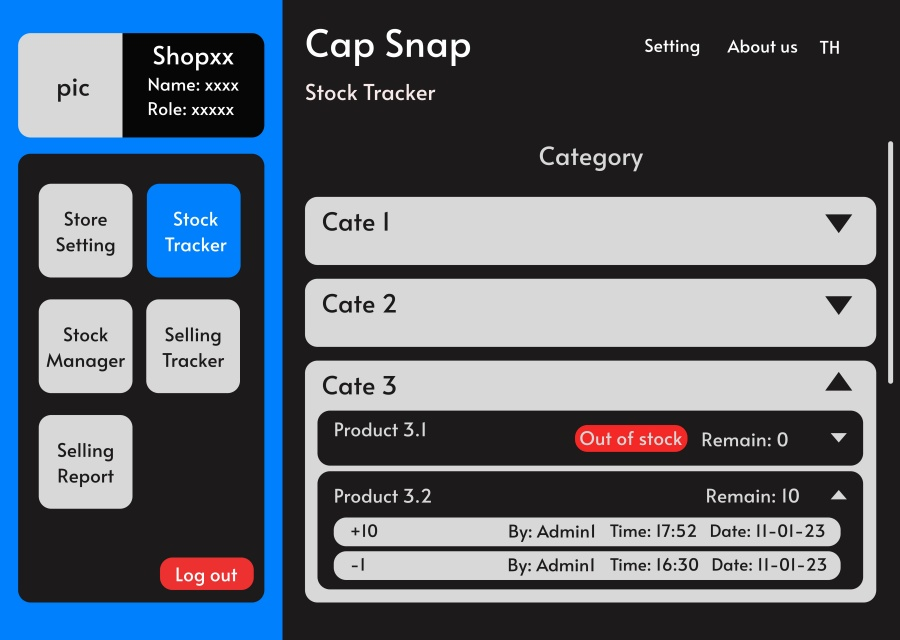
\includegraphics[scale=0.9]{pic/ui/5.jpg}
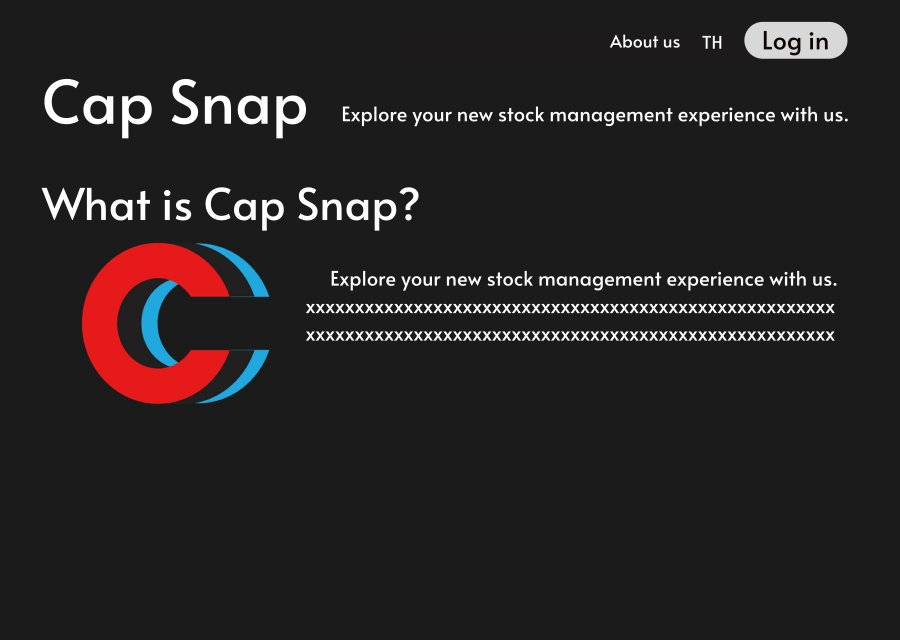
\includegraphics[scale=0.9]{pic/ui/6.jpg}
}\\
{
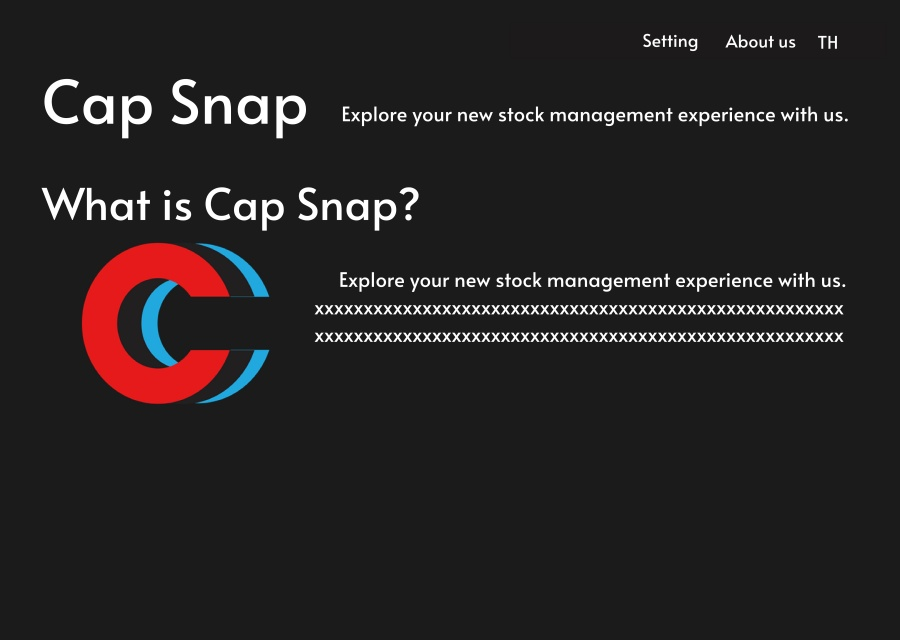
\includegraphics[scale=0.9]{pic/ui/7.jpg}
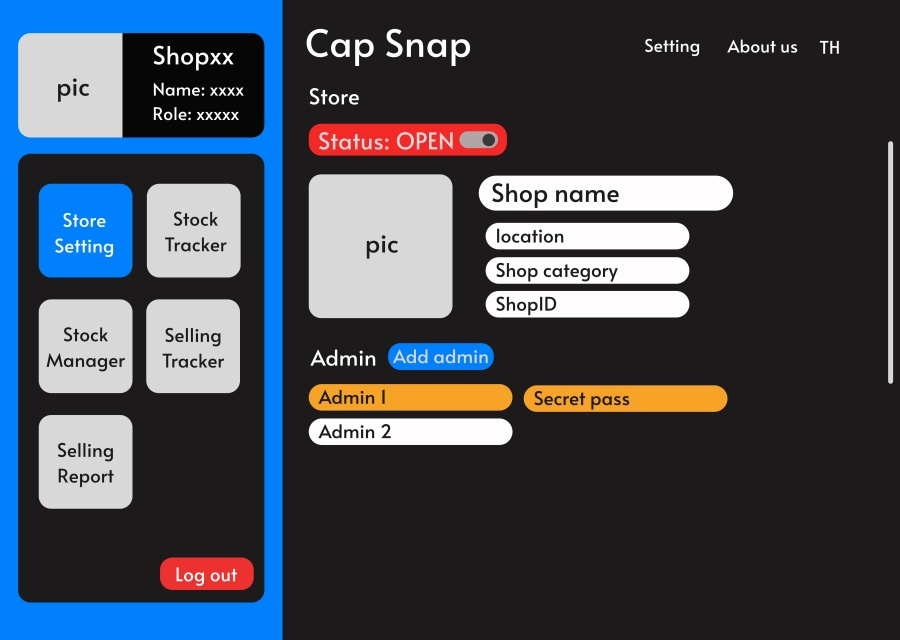
\includegraphics[scale=0.9]{pic/ui/8.jpg}
}\\
{
 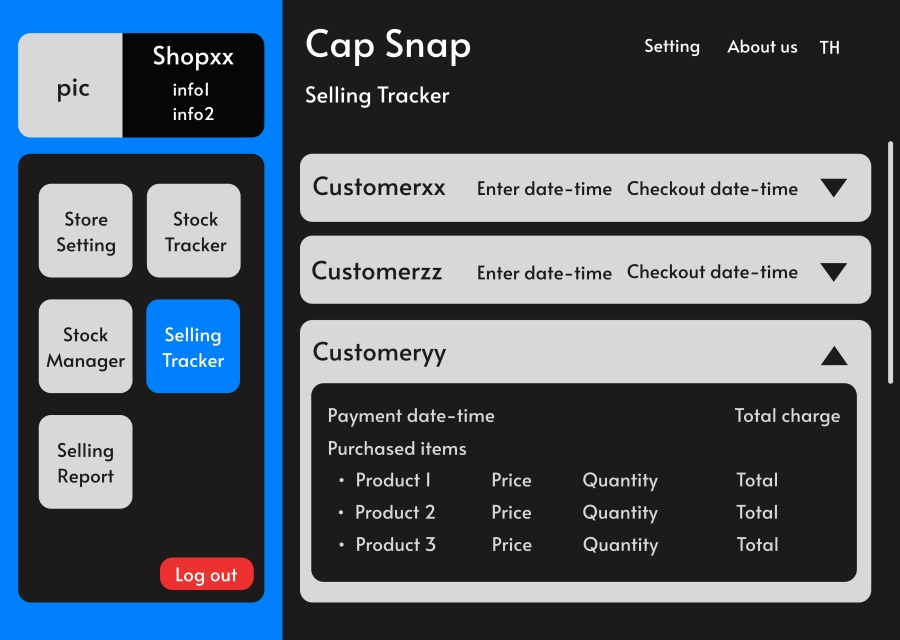
\includegraphics[scale=0.9]{pic/ui/9.jpg}
 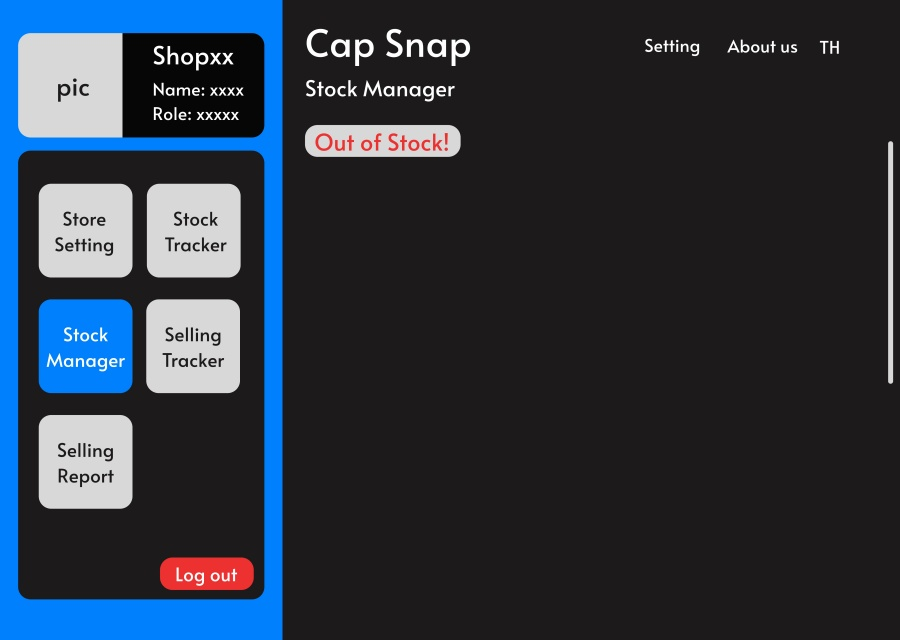
\includegraphics[scale=0.9]{pic/ui/10.jpg}
}\\
{
 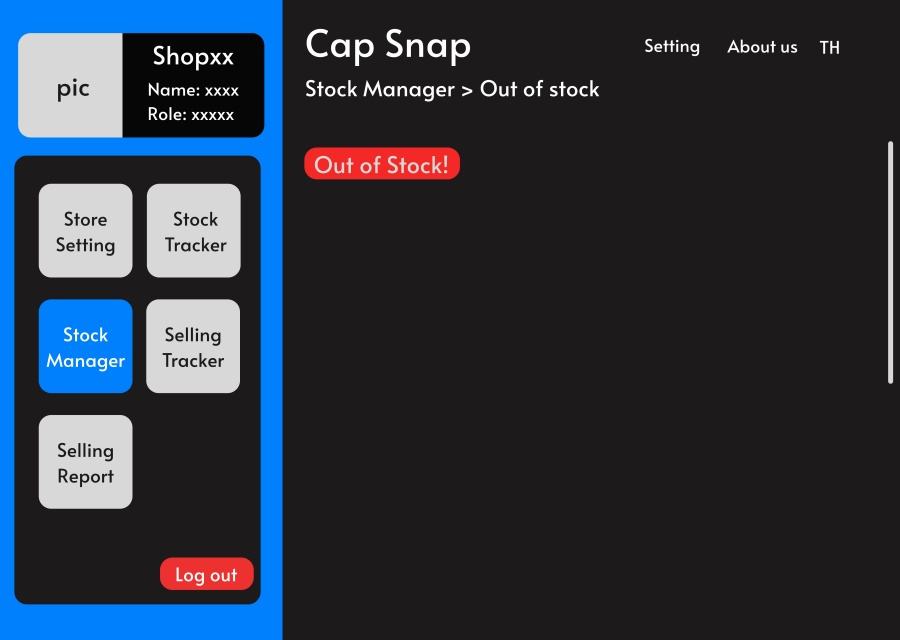
\includegraphics[scale=0.9]{pic/ui/11.jpg}
 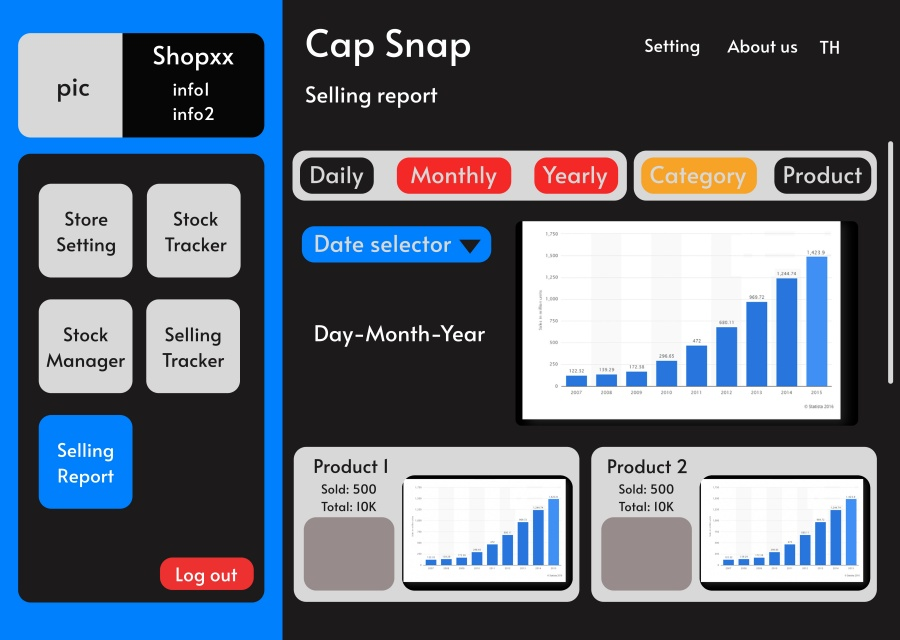
\includegraphics[scale=0.9]{pic/ui/12.jpg}
}
 
    
    
    % \end{center}


\ifproject
\chapter{\ifenglish Conclusions and Discussions\else บทสรุปและข้อเสนอแนะ\fi}

\section{\ifenglish Conclusions\else สรุปผล\fi}

% นศ. ควรสรุปถึงข้อจำกัดของระบบในด้านต่างๆ ที่ระบบมีในเนื้อหาส่วนนี้ด้วย

\section{\ifenglish Challenges\else ปัญหาที่พบและแนวทางการแก้ไข\fi}

% ในการทำโครงงานนี้ พบว่าเกิดปัญหาหลักๆ ดังนี้

\section{\ifenglish%
Suggestions and further improvements
\else%
ข้อเสนอแนะและแนวทางการพัฒนาต่อ
\fi
}

% ข้อเสนอแนะเพื่อพัฒนาโครงงานนี้ต่อไป มีดังนี้

\fi


% บรรณานุกรม 
% \bibliography{myReport}        

\ifproject
\normalspacing
\appendix
\chapter{The first appendix}

% \begin{figure}[h]
    \begin{center}
    % 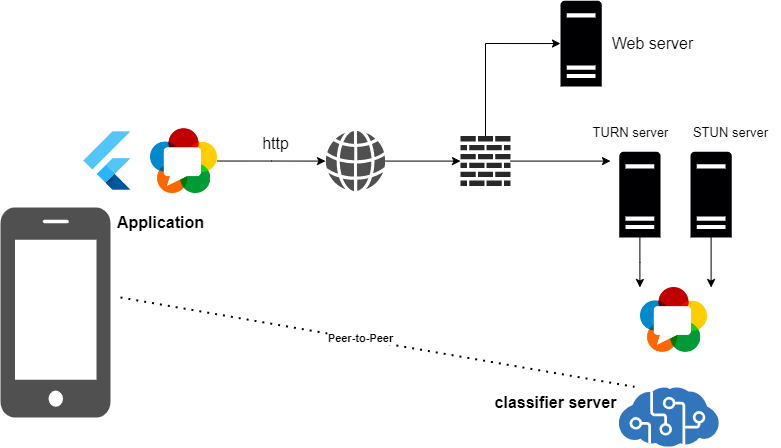
\includegraphics{pic/webrtc.png}
    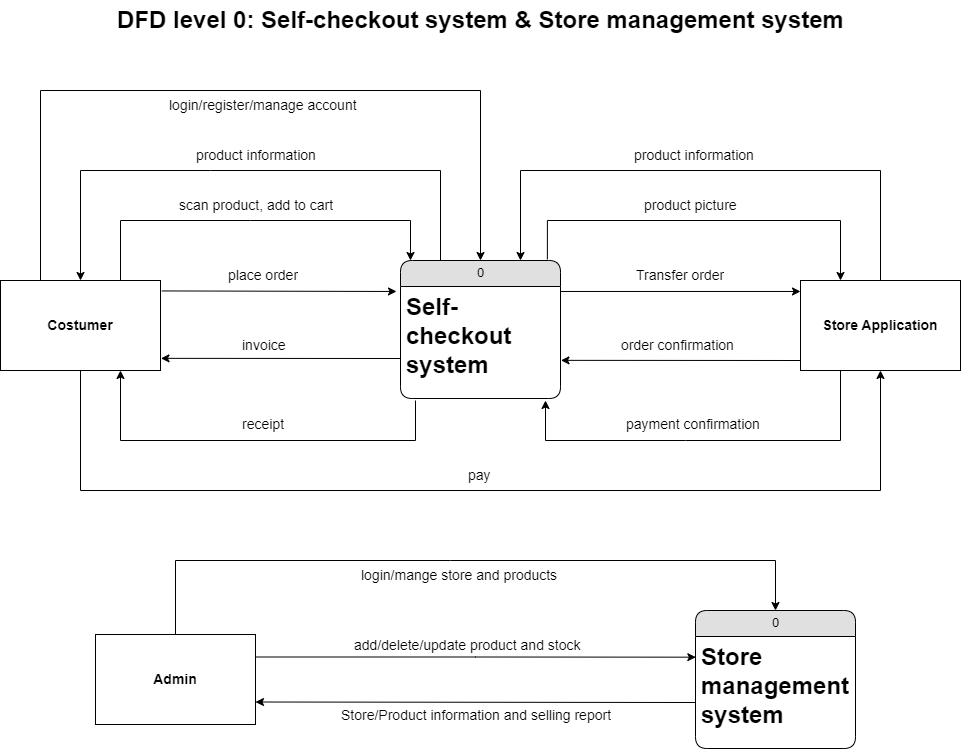
\includegraphics[scale=0.25]{pic/dataflow_p1.png}\\
    \vspace{2cm}
    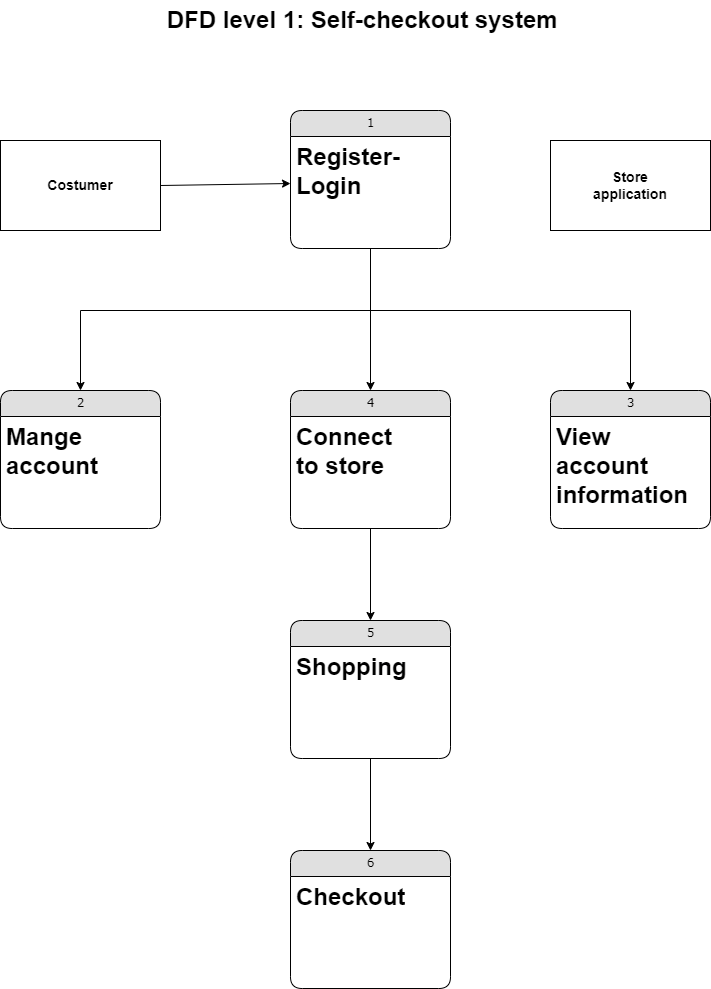
\includegraphics[scale=0.25]{pic/dataflow_p2.png}
    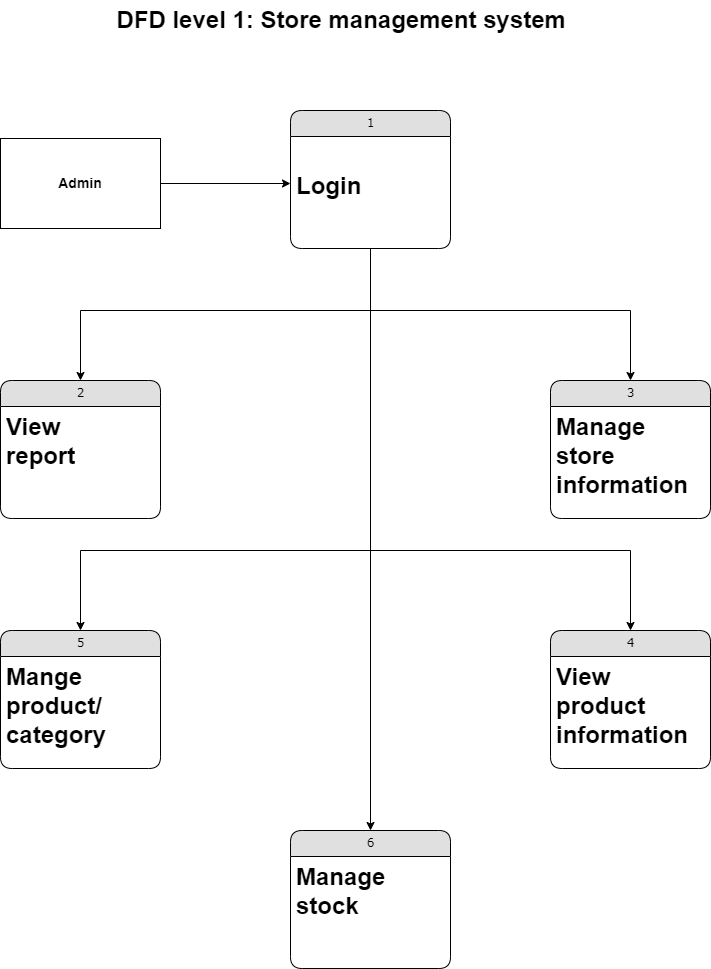
\includegraphics[scale=0.25]{pic/dataflow_p3.png}
    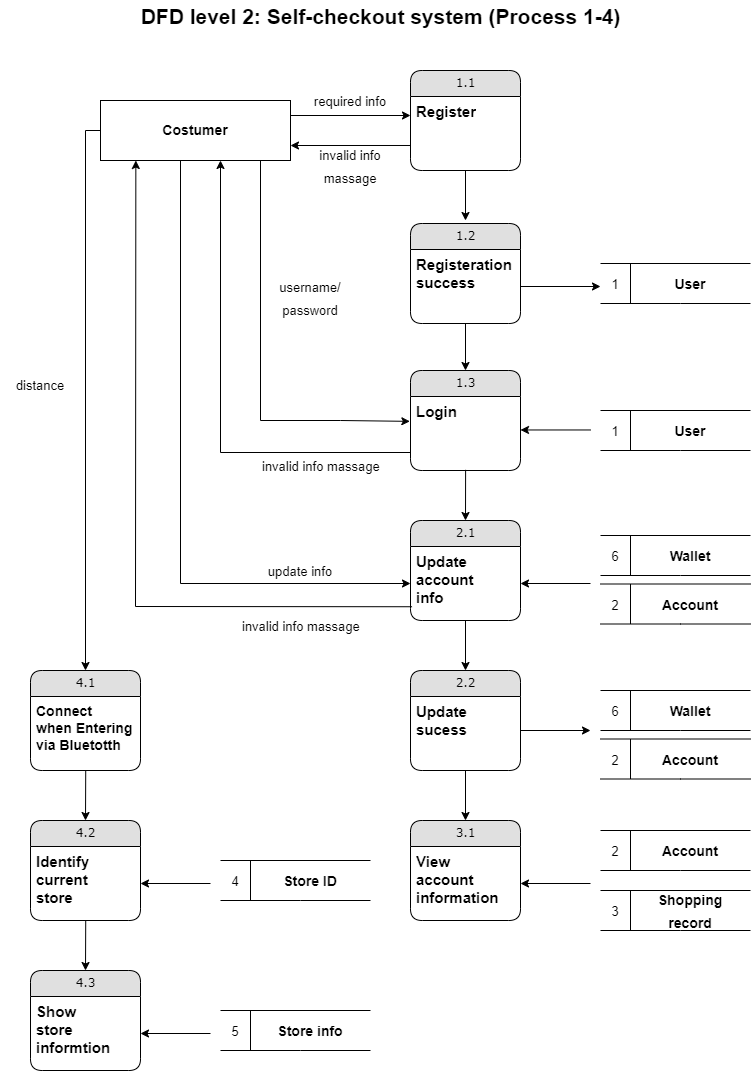
\includegraphics[scale=0.25]{pic/dataflow_p4.png}
    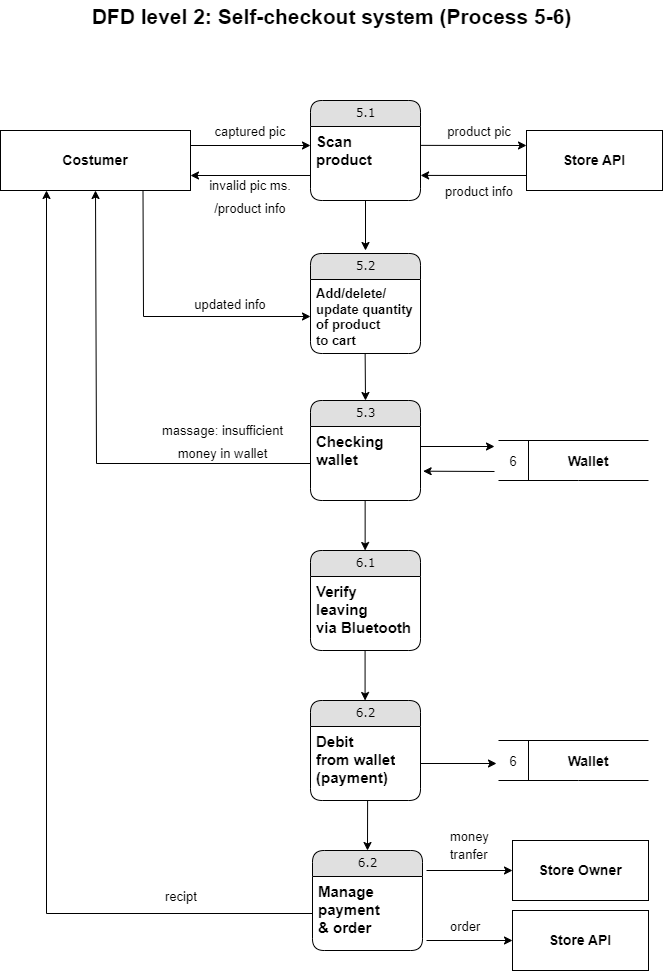
\includegraphics[scale=0.25]{pic/dataflow_p5.png}\\
    \vspace{2cm}
    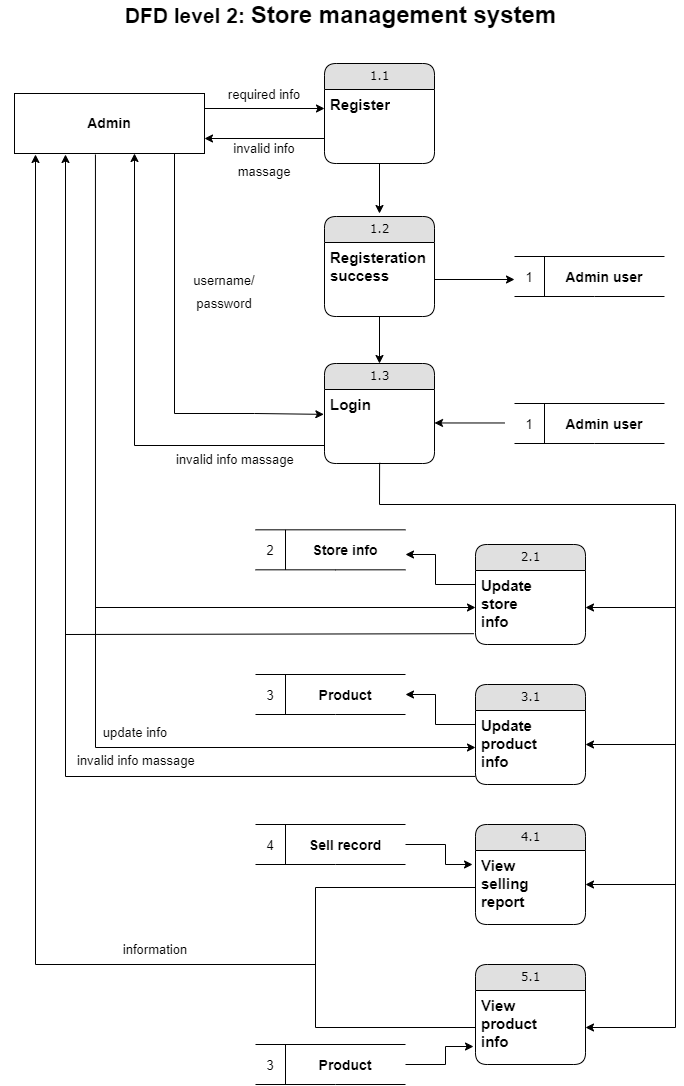
\includegraphics[scale=0.25]{pic/dataflow_p6.png}
    \end{center}
    
    % \caption[Data Flow Diagram all]{Data Flow Diagram all}
    % \label{fig:Data Flow Diagram all}
    % \end{figure}

% \section{Appendix section}

% Text for a section in the first appendix goes here.

% test ทดสอบฟอนต์ serif ภาษาไทย

% \textsf{test ทดสอบฟอนต์ sans serif ภาษาไทย}

% \verb+test ทดสอบฟอนต์ teletype ภาษาไทย+

% \texttt{test ทดสอบฟอนต์ teletype ภาษาไทย}

% \textbf{ตัวหนา serif ภาษาไทย \textsf{sans serif ภาษาไทย} \texttt{teletype ภาษาไทย}}

% \textit{ตัวเอียง serif ภาษาไทย \textsf{sans serif ภาษาไทย} \texttt{teletype ภาษาไทย}}

% \textbf{\textit{ตัวหนาเอียง serif ภาษาไทย \textsf{sans serif ภาษาไทย} \texttt{teletype ภาษาไทย}}}

% \url{https://www.example.com/test_ทดสอบ_url}

% \chapter{\ifenglish Manual\else คู่มือการใช้งานระบบ\fi}

% Manual goes here.


%% Display glossary (optional) -- need glossary option.
\ifglossary\glossarypage\fi

%% Display index (optional) -- need idx option.
\ifindex\indexpage\fi

\begin{biosketch}
\begin{center}
  \includegraphics[width=1.5in]{mugshot.jpg}
\end{center}
Your biosketch goes here. Make sure it sits inside
the \texttt{biosketch} environment.
\end{biosketch}
\fi % \ifproject
\end{document}
